\documentclass[12pt,a4paper]{standalone}
\usepackage{amssymb}
\usepackage{amsmath}
\usepackage{bm}
\usepackage{tikz}
\usetikzlibrary{arrows.meta}
\usetikzlibrary{arrows}
\usepackage{pstricks}
\usetikzlibrary{patterns}
\usetikzlibrary{fadings}
\usetikzlibrary{shapes.geometric}



\begin{document}
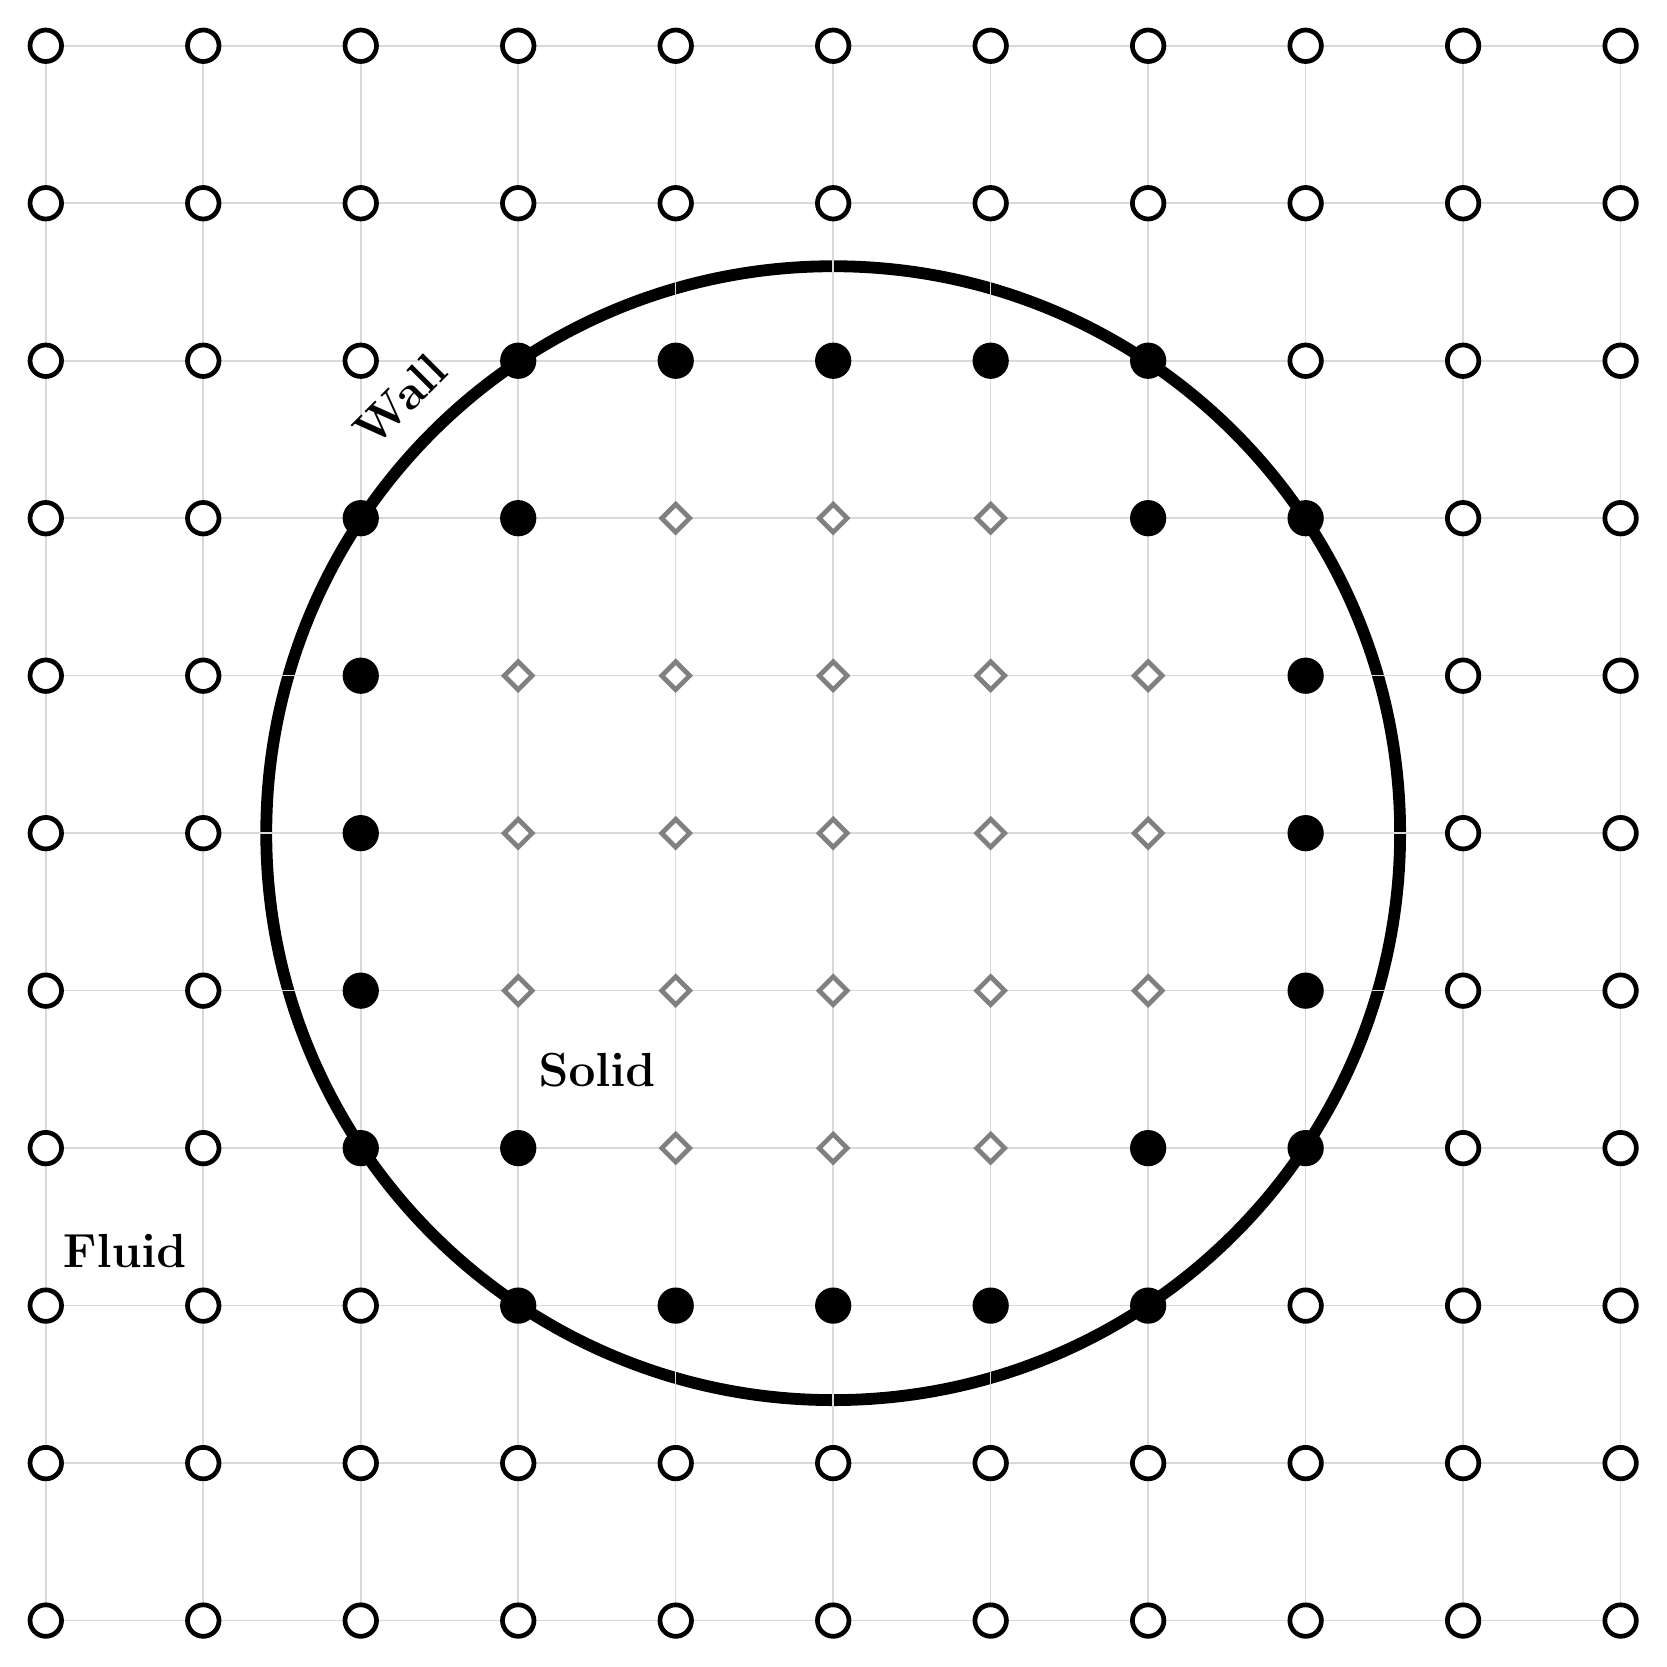
\begin{tikzpicture}[line width=0.6mm]

    \draw[thick,line width=1.5mm] (17.2,10) arc[start angle=0, end angle=360, radius=7.2];

    \draw[gray!30,solid,thick,line width=0.2mm] (0,0) -- (20,0);
    \draw[gray!30,solid,thick,line width=0.2mm] (0,2) -- (20,2);
    \draw[gray!30,solid,thick,line width=0.2mm] (0,4) -- (20,4);
    \draw[gray!30,solid,thick,line width=0.2mm] (0,6) -- (20,6);
    \draw[gray!30,solid,thick,line width=0.2mm] (0,8) -- (20,8);
    \draw[gray!30,solid,thick,line width=0.2mm] (0,10) -- (20,10);
    \draw[gray!30,solid,thick,line width=0.2mm] (0,12) -- (20,12);
    \draw[gray!30,solid,thick,line width=0.2mm] (0,14) -- (20,14);
    \draw[gray!30,solid,thick,line width=0.2mm] (0,16) -- (20,16);
    \draw[gray!30,solid,thick,line width=0.2mm] (0,18) -- (20,18);
    \draw[gray!30,solid,thick,line width=0.2mm] (0,20) -- (20,20);

    \draw[gray!30,solid,thick,line width=0.2mm] (0,0) -- (0,20);
    \draw[gray!30,solid,thick,line width=0.2mm] (2,0) -- (2,20);
    \draw[gray!30,solid,thick,line width=0.2mm] (4,0) -- (4,20);
    \draw[gray!30,solid,thick,line width=0.2mm] (6,0) -- (6,20);
    \draw[gray!30,solid,thick,line width=0.2mm] (8,0) -- (8,20);
    \draw[gray!30,solid,thick,line width=0.2mm] (10,0) -- (10,20);
    \draw[gray!30,solid,thick,line width=0.2mm] (12,0) -- (12,20);
    \draw[gray!30,solid,thick,line width=0.2mm] (14,0) -- (14,20);
    \draw[gray!30,solid,thick,line width=0.2mm] (16,0) -- (16,20);
    \draw[gray!30,solid,thick,line width=0.2mm] (18,0) -- (18,20);
    \draw[gray!30,solid,thick,line width=0.2mm] (20,0) -- (20,20);

    %First column
    \draw[black,fill=white] (0,0)node[]{} circle(0.2cm);
    \draw[black,fill=white] (0,2)node[]{} circle(0.2cm);
    \draw[black,fill=white] (0,4)node[]{} circle(0.2cm);
    \draw[black,fill=white] (0,6)node[]{} circle(0.2cm);
    \draw[black,fill=white] (0,8)node[]{} circle(0.2cm);
    \draw[black,fill=white] (0,10)node[]{} circle(0.2cm);
    \draw[black,fill=white] (0,12)node[]{} circle(0.2cm);
    \draw[black,fill=white] (0,14)node[]{} circle(0.2cm);
    \draw[black,fill=white] (0,16)node[]{} circle(0.2cm);
    \draw[black,fill=white] (0,18)node[]{} circle(0.2cm);
    \draw[black,fill=white] (0,20)node[]{} circle(0.2cm);

    %second column
    \draw[black,fill=white] (2,0)node[]{} circle(0.2cm);
    \draw[black,fill=white] (2,2)node[]{} circle(0.2cm);
    \draw[black,fill=white] (2,4)node[]{} circle(0.2cm);
    \draw[black,fill=white] (2,6)node[]{} circle(0.2cm);
    \draw[black,fill=white] (2,8)node[]{} circle(0.2cm);
    \draw[black,fill=white] (2,10)node[]{} circle(0.2cm);
    \draw[black,fill=white] (2,12)node[]{} circle(0.2cm);
    \draw[black,fill=white] (2,14)node[]{} circle(0.2cm);
    \draw[black,fill=white] (2,16)node[]{} circle(0.2cm);
    \draw[black,fill=white] (2,18)node[]{} circle(0.2cm);
    \draw[black,fill=white] (2,20)node[]{} circle(0.2cm);

    %Third column
    \draw[black,fill=white] (4,0)node[]{} circle(0.2cm);
    \draw[black,fill=white] (4,2)node[]{} circle(0.2cm);
    \draw[black,fill=white] (4,4)node[]{} circle(0.2cm);
    \draw[black,fill=black] (4,6)node[]{} circle(0.2cm);
    \draw[black,fill=black] (4,8)node[]{} circle(0.2cm);
    \draw[black,fill=black] (4,10)node[]{} circle(0.2cm);
    \draw[black,fill=black] (4,12)node[]{} circle(0.2cm);
    \draw[black,fill=black] (4,14)node[]{} circle(0.2cm);
    \draw[black,fill=white] (4,16)node[]{} circle(0.2cm);
    \draw[black,fill=white] (4,18)node[]{} circle(0.2cm);
    \draw[black,fill=white] (4,20)node[]{} circle(0.2cm);

    %fourth column
    \draw[black,fill=white] (6,0)node[]{} circle(0.2cm);
    \draw[black,fill=white] (6,2)node[]{} circle(0.2cm);
    \draw[black,fill=black] (6,4)node[]{} circle(0.2cm);
    \draw[black,fill=black] (6,6)node[]{} circle(0.2cm);
    \node [draw, gray, fill=white,diamond, aspect=1,scale=0.8] at (6,8) {};
    \node [draw, gray, fill=white,diamond, aspect=1,scale=0.8] at (6,10) {};
    \node [draw, gray, fill=white,diamond, aspect=1,scale=0.8] at (6,12) {};
    \draw[black,fill=black] (6,14)node[]{} circle(0.2cm);
    \draw[black,fill=black] (6,16)node[]{} circle(0.2cm);
    \draw[black,fill=white] (6,18)node[]{} circle(0.2cm);
    \draw[black,fill=white] (6,20)node[]{} circle(0.2cm);

    %fifth column
    \draw[black,fill=white] (8,0)node[]{} circle(0.2cm);
    \draw[black,fill=white] (8,2)node[]{} circle(0.2cm);
    \draw[black,fill=black] (8,4)node[]{} circle(0.2cm);
    \node [draw, gray, fill=white,diamond, aspect=1,scale=0.8] at (8,6) {};
    \node [draw, gray, fill=white,diamond, aspect=1,scale=0.8] at (8,8) {};
    \node [draw, gray, fill=white,diamond, aspect=1,scale=0.8] at (8,10) {};
    \node [draw, gray, fill=white,diamond, aspect=1,scale=0.8] at (8,12) {};
    \node [draw, gray, fill=white,diamond, aspect=1,scale=0.8] at (8,14) {};
    \draw[black,fill=black] (8,16)node[]{} circle(0.2cm);
    \draw[black,fill=white] (8,18)node[]{} circle(0.2cm);
    \draw[black,fill=white] (8,20)node[]{} circle(0.2cm);

    %sixth column
    \draw[black,fill=white] (10,0)node[]{} circle(0.2cm);
    \draw[black,fill=white] (10,2)node[]{} circle(0.2cm);
    \draw[black,fill=black] (10,4)node[]{} circle(0.2cm);
    \node [draw, gray, fill=white,diamond, aspect=1,scale=0.8] at (10,6) {};
    \node [draw, gray, fill=white,diamond, aspect=1,scale=0.8] at (10,8) {};
    \node [draw, gray, fill=white,diamond, aspect=1,scale=0.8] at (10,10) {};
    \node [draw, gray, fill=white,diamond, aspect=1,scale=0.8] at (10,12) {};
    \node [draw, gray, fill=white,diamond, aspect=1,scale=0.8] at (10,14) {};
    \draw[black,fill=black] (10,16)node[]{} circle(0.2cm);
    \draw[black,fill=white] (10,18)node[]{} circle(0.2cm);
    \draw[black,fill=white] (10,20)node[]{} circle(0.2cm);

    \draw[black,fill=white] (12,0)node[]{} circle(0.2cm);
    \draw[black,fill=white] (12,2)node[]{} circle(0.2cm);
    \draw[black,fill=black] (12,4)node[]{} circle(0.2cm);
    \node [draw, gray, fill=white,diamond, aspect=1,scale=0.8] at (12,6) {};
    \node [draw, gray, fill=white,diamond, aspect=1,scale=0.8] at (12,8) {};
    \node [draw, gray, fill=white,diamond, aspect=1,scale=0.8] at (12,10) {};
    \node [draw, gray, fill=white,diamond, aspect=1,scale=0.8] at (12,12) {};
    \node [draw, gray, fill=white,diamond, aspect=1,scale=0.8] at (12,14) {};
    \draw[black,fill=black] (12,16)node[]{} circle(0.2cm);
    \draw[black,fill=white] (12,18)node[]{} circle(0.2cm);
    \draw[black,fill=white] (12,20)node[]{} circle(0.2cm);

    \draw[black,fill=white] (14,0)node[]{} circle(0.2cm);
    \draw[black,fill=white] (14,2)node[]{} circle(0.2cm);
    \draw[black,fill=black] (14,4)node[]{} circle(0.2cm);
    \draw[black,fill=black] (14,6)node[]{} circle(0.2cm);
    \node [draw, gray, fill=white,diamond, aspect=1,scale=0.8] at (14,8) {};
    \node [draw, gray, fill=white,diamond, aspect=1,scale=0.8] at (14,10) {};
    \node [draw, gray, fill=white,diamond, aspect=1,scale=0.8] at (14,12) {};
    \draw[black,fill=black] (14,14)node[]{} circle(0.2cm);
    \draw[black,fill=black] (14,16)node[]{} circle(0.2cm);
    \draw[black,fill=white] (14,18)node[]{} circle(0.2cm);
    \draw[black,fill=white] (14,20)node[]{} circle(0.2cm);

    \draw[black,fill=white] (16,0)node[]{} circle(0.2cm);
    \draw[black,fill=white] (16,2)node[]{} circle(0.2cm);
    \draw[black,fill=white] (16,4)node[]{} circle(0.2cm);
    \draw[black,fill=black] (16,6)node[]{} circle(0.2cm);
    \draw[black,fill=black] (16,8)node[]{} circle(0.2cm);
    \draw[black,fill=black] (16,10)node[]{} circle(0.2cm);
    \draw[black,fill=black] (16,12)node[]{} circle(0.2cm);
    \draw[black,fill=black] (16,14)node[]{} circle(0.2cm);
    \draw[black,fill=white] (16,16)node[]{} circle(0.2cm);
    \draw[black,fill=white] (16,18)node[]{} circle(0.2cm);
    \draw[black,fill=white] (16,20)node[]{} circle(0.2cm);

    \draw[black,fill=white] (18,0)node[]{} circle(0.2cm);
    \draw[black,fill=white] (18,2)node[]{} circle(0.2cm);
    \draw[black,fill=white] (18,4)node[]{} circle(0.2cm);
    \draw[black,fill=white] (18,6)node[]{} circle(0.2cm);
    \draw[black,fill=white] (18,8)node[]{} circle(0.2cm);
    \draw[black,fill=white] (18,10)node[]{} circle(0.2cm);
    \draw[black,fill=white] (18,12)node[]{} circle(0.2cm);
    \draw[black,fill=white] (18,14)node[]{} circle(0.2cm);
    \draw[black,fill=white] (18,16)node[]{} circle(0.2cm);
    \draw[black,fill=white] (18,18)node[]{} circle(0.2cm);
    \draw[black,fill=white] (18,20)node[]{} circle(0.2cm);

    \draw[black,fill=white] (20,0)node[]{} circle(0.2cm);
    \draw[black,fill=white] (20,2)node[]{} circle(0.2cm);
    \draw[black,fill=white] (20,4)node[]{} circle(0.2cm);
    \draw[black,fill=white] (20,6)node[]{} circle(0.2cm);
    \draw[black,fill=white] (20,8)node[]{} circle(0.2cm);
    \draw[black,fill=white] (20,10)node[]{} circle(0.2cm);
    \draw[black,fill=white] (20,12)node[]{} circle(0.2cm);
    \draw[black,fill=white] (20,14)node[]{} circle(0.2cm);
    \draw[black,fill=white] (20,16)node[]{} circle(0.2cm);
    \draw[black,fill=white] (20,18)node[]{} circle(0.2cm);
    \draw[black,fill=white] (20,20)node[]{} circle(0.2cm);

    \draw (1,4.7)node[]{{\LARGE{\textbf{Fluid}}}};
    \draw (7,7)node[]{{\LARGE{\textbf{Solid}}}};
    \draw (4.5,15.5)node[rotate=45]{{\LARGE{\textbf{Wall}}}};

    % \draw[dashed,thick,line width=0.2mm] (4,2) -- (7.7,7.4);

    % \draw[gray,solid,thick,line width=0.2mm] (0,0) -- (13,0);
    % \draw[gray,solid,thick,line width=0.2mm] (1,2) -- (13,2);
    % \draw[gray,solid,thick,line width=0.2mm] (1,4) -- (13,4);
    % \draw[gray,solid,thick,line width=0.2mm] (1,6) -- (13,6);
    % \draw[gray,solid,thick,line width=0.2mm] (1,8) -- (13,8);
    %
    % \draw[gray,solid,thick,line width=0.2mm] (2,-1) -- (2,9);
    % \draw[gray,solid,thick,line width=0.2mm] (4,-1) -- (4,9);
    % \draw[gray,solid,thick,line width=0.2mm] (6,-1) -- (6,9);
    % \draw[gray,solid,thick,line width=0.2mm] (8,-1) -- (8,9);
    % \draw[gray,solid,thick,line width=0.2mm] (10,-1) -- (10,9);
    % \draw[gray,solid,thick,line width=0.2mm] (12,-1) -- (12,9);

    % \draw[thick,line width=1mm] (8.2,-0.4) arc[start angle=15, end angle=85, radius=8];
    % \draw[pattern=north west lines, pattern color=white] (6,4) rectangle (8,6);
    % \draw[pattern=north east lines, pattern color=gray] (6,6) rectangle (8,8);

    % %top first row
    % \draw[black,fill=white] (2,8)node[]{} circle(0.2cm);
    % \draw[black,fill=white] (4,8)node[]{} circle(0.15cm);
    % \draw[black,fill=white] (6,8)node[]{} circle(0.15cm);
    % \draw[black,fill=white] (8,8)node[]{} circle(0.15cm);
    % \draw[black,fill=white] (10,8)node[]{} circle(0.15cm);
    % \draw[black,fill=white] (12,8)node[]{} circle(0.15cm);
    %
    % %top second row
    % \draw[black,fill=white] (2,6)node[]{} circle(0.15cm);
    % \draw[black,fill=white] (4,6)node[]{} circle(0.15cm);
    % \draw[black,fill=white] (6,6)node[]{} circle(0.15cm);
    % \draw[black,fill=white] (8,6)node[]{} circle(0.15cm);
    % \draw[black,fill=white] (10,6)node[]{} circle(0.15cm);
    % \draw[black,fill=white] (12,6)node[]{} circle(0.15cm);
    %
    % %top third row
    % \draw[black,fill=black] (2,4)node[]{} circle(0.15cm);
    % \draw[black,fill=black] (4,4)node[]{} circle(0.15cm);
    % \draw[black,fill=white] (6,4)node[]{} circle(0.15cm);
    % \draw[black,fill=white] (8,4)node[]{} circle(0.15cm);
    % \draw[black,fill=white] (10,4)node[]{} circle(0.15cm);
    % \draw[black,fill=white] (12,4)node[]{} circle(0.15cm);
    %
    % %top fourth row
    % \draw[black,fill=black] (4,2)node[]{} circle(0.15cm);
    % \draw[black,fill=black] (6,2)node[]{} circle(0.15cm);
    % \draw[black,fill=white] (8,2)node[]{} circle(0.15cm);
    % \draw[black,fill=white] (10,2)node[]{} circle(0.15cm);
    % \draw[black,fill=white] (12,2)node[]{} circle(0.15cm);
    %
    % %top fifth row
    % \draw[black,fill=black] (6,0)node[]{} circle(0.15cm);
    % \draw[black,fill=black] (8,0)node[]{} circle(0.15cm);
    % \draw[black,fill=white] (10,0)node[]{} circle(0.15cm);
    % \draw[black,fill=white] (12,0)node[]{} circle(0.15cm);

    % \node [draw, fill=gray,diamond, aspect=1,scale=0.7] at (5.22,3.78) {};
    % \node [draw, fill=gray,diamond, aspect=1,scale=0.7] at (6.4,5.5) {};
    % \node [draw, fill=gray,diamond, aspect=1,scale=0.7] at (7.7,7.4) {};
    %
    % \draw (7,5.2)node[]{\large{$\bm{P_{f1}}$}};
    % \draw (8.4,7.4)node[]{\large{$\bm{P_{f2}}$}};
    %
    %
    % \draw (5.7,5)node[]{\Large{$\delta_r$}};
    % \draw (7,7)node[]{\Large{$\delta_r$}};
    % \draw (4.3,3.2)node[]{\Large{$\Delta$}};
    %
    %
    % \draw (4.3,1.6)node[]{\Large{$\bm{b}$}};
    % \draw (2.7,1.5)node[]{{\textbf{boundary}}};
    % \draw (2.9,1)node[]{\textbf{node}};

    % \draw (5.8,4.3)node[]{\large{$\bm{f}$}};
    % \draw (6.8,3.6)node[]{\textbf{fluid}};
    % \draw (6.8,3.1)node[]{\textbf{node}};

    % \draw (7.6,6.3)node[]{\large{$\bm{ff}$}};

    % \draw (5.2,4.3)node[]{\Large{$\bm{w}$}};
    % \draw (5.4,3)node[]{{\textbf{wall}}};
    % \draw (5.64,2.5)node[]{{\textbf{point}}};
    %
    % \draw (1.9,4.7)node[]{{\textbf{physical}}};
    % \draw (2.4,4.25)node[]{{\textbf{boundary}}};

\end{tikzpicture}

\end{document}

